\begin{figure*}[tp]
\centering
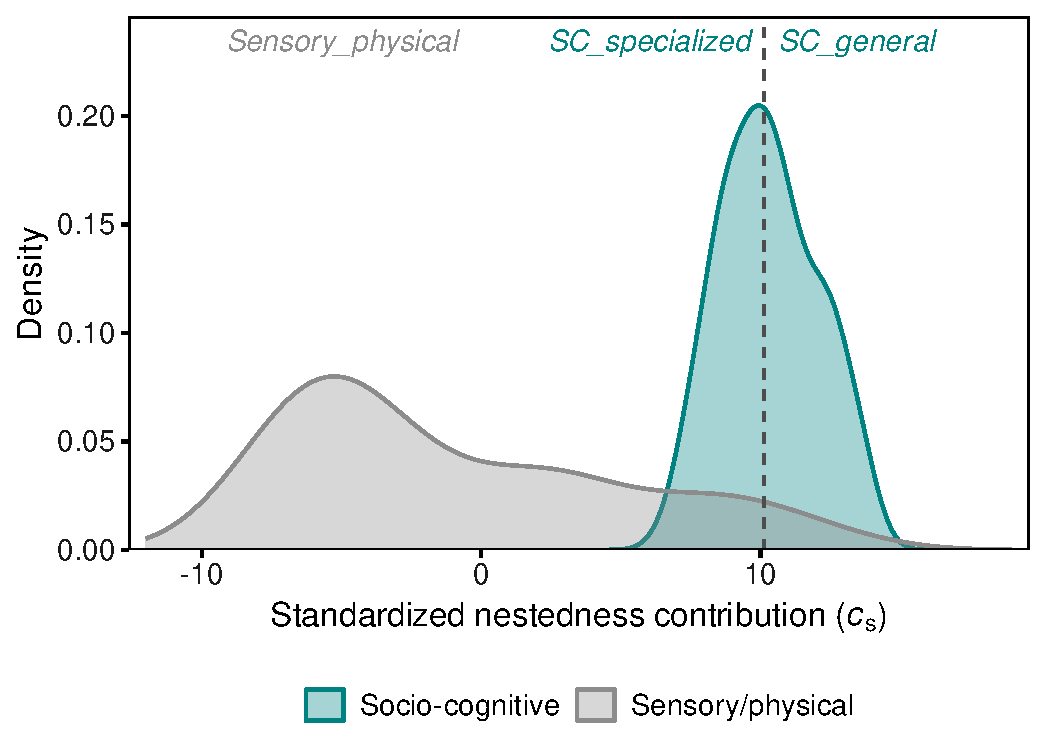
\includegraphics[width=0.65\textwidth]{figures/fig_S2_cs_distribution.pdf}
\caption{\textbf{Distribution of nestedness contribution scores ($c_s$) by functional domain.} Each curve shows the kernel density of $c_s$ across skills within one functional domain. Within the socio-cognitive domain (teal), all skills have $c_s > 0$ in our data; the dashed vertical line marks the within-domain median, which defines the boundary between specialized socio-cognitive (left of median, $n = 48$) and general socio-cognitive (right of median, $n = 49$) skills. Within the sensory-physical domain (gray), $c_s$ values are negative throughout, confirming the absence of a high-nestedness sensory-physical cluster. O*NET 2015.}
\label{fig:SI_cs_distribution}
\end{figure*}
